
 \section{ Model Background}

 \subsection{ Fractional Occupancy of Morphogen Binding to DNA binding Site}

The binding process is modeled using a first order rate law, where M is morphogen and B is the Binding site of DNA, and MB is the complex:
\begin{equation}\label{}
    \frac{d [MB)]}{dt}= k_{on}[M][B] - k_{off}[MB],
\end{equation}
where the brackets [ ] denote concentrations, and $k_{on}$ is diffusion limited on rate,  and $k_{off}$ is the off rate that is determined by the electrostatic interactions and will vary between morphogens.  Using chemical reaction notation, we can write the above rate law as:
\begin{equation}\label{}
    [M] + [B] \Leftrightarrow [MB].
\end{equation}
In equilibrium we have:
\begin{equation}\label{ka}
  K_{a} =  \frac{[MB]}{[M][B]}= \frac{k_{on} }{k_{off}},
\end{equation}
where the $K_{a}$ is the association constant (binding constant).
The Binding site is either occupied ($o$) or unoccupied ($u$) hence the total ($t$) amount of B is conserved :
\begin{equation}\label{}
    B_{t} = B_{u} + B_{o}
\end{equation}
From this equation one is able to construct a Binomial probability space\footnote[2]{If we encode the bound state and unbound state in the Bernoulli Random variable (i.e. 1,0) we have: $E(X) = \mu = \sum_i X_i P_i = 1 P + 0 (1-P) $} \footnote[3]{ $\sigma^2 (X) =\sum_i (X_i-\mu)^2 P_i = (1-P)^2P + (0-P)^2(1-P) = (1-P)P $ }.  The fraction of occupied binding site $B$ determines the distribution's parameter $P$:
\begin{equation}\label{}
   P = \frac{B_{o}}{B_{t}}
\end{equation}
which can be rearranged in terms of the concentrations (i.e. [MB] and [B]):
\begin{equation}\label{Zb}
    \frac{B_{o}}{B_{t}} =\frac{[MB]}{[MB] + [B]}
\end{equation}

\begin{equation}\label{}
    P =\frac{[MB]}{[MB] + [B]} = \frac{K_{a}[M]}{1+K_{a}[M]}.
\end{equation}
Again, $K_a$ is the association constant of the morphogen, $M$, to the binding site $B$.  Previously we have denoted this constant as $K(S)$, where $S$ is a DNA sequence that functions as a binding site for the morphogen. 

\subsection{ Fractional occupancy of CRMs containing multiple binding sites }


Given that most regulatory sequences have multiple binding sites for multiple different morphogens one has a master equation governing the binding process, a set of coupled differential equations.  Here, again, we will assume the binding process has equilibrated, and hence we simply must enumerate the states (configurations of bound and unbound sites) of the many-binding site system.  For independent binding this is simply multinomial process (where the 'multi' aspect accounts for the different types of transcription factors binding to the CRM).  For example, for a single type of transcription factor binding, to n binding sites within a CRM, one has a binomial process governed by the partition function $(1+q)^n$, as discussed in the introduction of the dissertation.  Hence, the probability of k bound factors is simply $P(k) =  {n \choose k}p^k(1-p)^{n-k}$, where $p$ is a Boltzmann probability for a single bound site, and $p^k(1-p)^{n-k}$ is joint probability of a particular binding configuration (\emph{which} configuration is irrelevant for the case of identical sites binding the same morphogen).  However, for the case of dependencies between the sites, we can not factorize the joint distribution over binding sites (\textit{i.e.} $(1+q)^n$ is a factorization of the partition function, and hence factorization of the joint distribution).  Furthermore, for the case where the sites are not identical, such as in CRMs that have heterogenous binding sites due to each transcription factor's DNA sequence specificity, we do not simply have one Boltzmann probability $p$ for all the sites.  Hence, each site will need a distinguishing notation.  Furthermore, the number of sites $n$ is not always known.  Hence, in some cases, one must discover $n$ sites, by 'annotating' the CRM which defines the coordinates of each transcription factor's sites and their corresponding energy.  In the next three sections we will describe a notation that is a mixture of notations used for Hidden Markov Models (HMM) and Lattice Gases (Ising Models) that is hybridization of the notations from Segal et.al.\cite{pmid18172436} (HMM notation) and the notation used by both Xin He et.al.\cite{pmid20862354}\cite{pmid19956545}.  Hereafter these notations will simply be referred to as Segal's notation or Xin's notation.  The reason for the hybridization is because our model was originally based on the Segal's paper, which latter was merged with work from Xin He (who collaborated with others in Saurabh Sinha's lab and S. Zhong's lab), by usng Xin's GEMSTAT and STAP C++ programs as libraries for implementation of our model.

\subsection{Segal's Hidden Markov Model}     

 If one does not know the binding sites \textit{a priori} of a CRM then one could take all possible positions within the sequence as the start of a new binding site as in figure \ref{sb}, where the PWM (see chapter 2) scores each position of the sequence as a potential binding site, thereby creating a list of binding energies ordered according to the position within the CRM.  Repeating this for each morphogen's PWM, and by stacking the lists on top of each other, results in a matrix of energy scores that is useful for computation of the partition function through the forward algorithm from Hidden Markov Models (HMMs).  
 
 The partition function of the many body system requires the addition of the statistical weight (see the Boltzmann factor in equation \ref{wc}) from each possible 'path' through the matrix.  Each 'path' through the matrix represents a 'configuration' as in figure \ref{configurationMatrixI}.
\begin{figure}
  % Requires \usepackage{graphicx}
  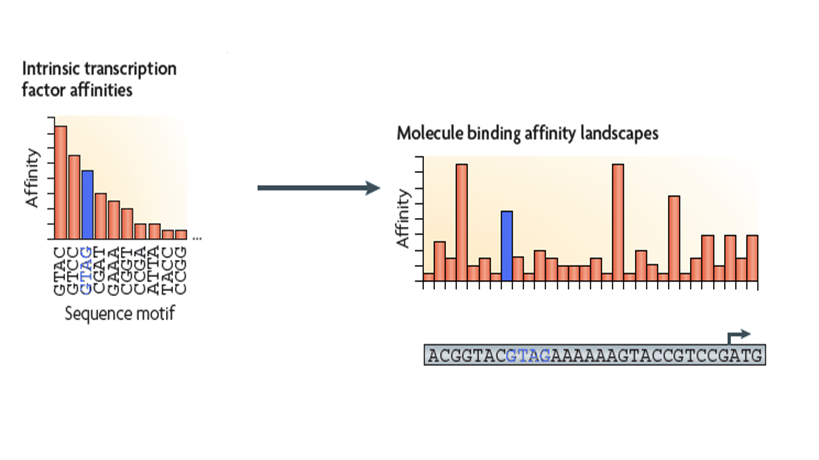
\includegraphics[width=1\textwidth]{segalblandscape}\\
  \caption{Widom, Segal Nature Review Genetics; "motif" denotes path through the PWM\cite{pmid19506578}}\label{sb}
\end{figure}
The partition function can be calculated by recursively moving through the matrix elements, in a way that is similar in spirit to standard algorithms of multiple sequence alignment\cite{BSA}, where we can think of each configuration as a possible way to 'align' each motif (PWM) to the CRM.  The variant of HMM's forward algorithm approach used by Segal for computing the partition function of all paths (configurations) is discussed in his supplementary material. 
\subsection{ Enumerating the configurations of a CRM sequence }

 Here we will introduce a notation for the weights of many-binding site systems.  First, let $P(c)$, be the probability of a particular configuration (c) occurring
\begin{equation}\label{mbody}
    P(c) = \frac{W(c)}{\Sigma_c W(c)},
\end{equation}
where $ W(c)$ is the boltzmann factor or weight of the binding configuration, which is a list of occupations for each binding site locus within the CRM, where the occupation is either bound or unbound.   Using the notation of Xin, from Sinha lab ( which was using Buchler's model as a guide\cite{pmid20862354}\cite{pmid12702751}, a notation used by Terrell Hill that I followed in the Introduction of the Dissertation), we have:
\begin{equation}\label{wc}
    W(c)=  [\prod_i^N q(x)_{tf(i)} ] [\prod_{j}^{N-1} \omega_{tf(i),tf(j)}(d)]
\end{equation}
Here we have $N$ bound transcription factors, where $q(x)_{tf(i)}$ is the weight of the transcription factor for the ith binding site ($tf(i)$) that is $\textbf{bound}$ at position $x$ of the sequence, 
\begin{equation}\label{partitionf}
    q(x)_{tf(i)} = K_{s(x)}^{tf(i)} [tf(i)]
\end{equation}
Here $ K_{s(x)}^{tf{i}}$ is the equilibrium constant $K_a$ from equation \eqref{ka} for the binding site sequence $s$ binding by transcription factor $i$.  And $\omega_{i,j}$ is the interaction between the two $\textbf{bound}$ factors $tf(i),tf(j)$, where we have one less nearest neighbor interaction than the number of bound factors.  And $d$ is the distance separating factor $tf(i)$ from factor $tf(j)$ in units of base pairs ( $d = x(tf(i)) - x(tf(j))$ where $x(tf(i))$ is the sequence coordinate of factor $tf(i)$).
\subsection{The configuration vector nomenclature}

 Here we have used 'c' to denote the binding configuration of bound and unbound factors on the CRM following the symbol Segal used to denote the configuration, and we have used a map $tf(i)$ to link each binding site i to a transcription factor.  This map is similar to notation used by Segal, where he explicitly denotes the type of transcription factor at each bound site.
 
  Xin used a configuration vector, $\sigma$, which had indicator variables $\sigma_i$ for ith componenet of their configuration vector, where the ith component was the ith binding 'site'.  Xin's notation is elegant, in that every 'site' in their model is clearly represented in their configuration vector by the occupancy of the ith component of the vector.  
  
  Segal's notation does not display all the possible bound and unbound positions in the configuration (since there is a background occupancy in his model that causes unbound sequence to have a Boltzmann weight of 1.).  I have tried to stick to Segal's notation for a configuration by only displaying bound factors in the Boltzmann weight of a configuration, and by denoting explicitly the type of transcription factor at each bound site.  However, Segal's notation is based only on the CRM sequence, he does not actually have a 'site' notation, since every possible position in the CRM is considered a binding site for each transcription factor, and he simply looks at all the possible ways that coordinately regulating transcription factors could form monolayers on the CRM, without overlapping one another.  Hence, in Segal's notation, there really is no notion of a 'functional' site, as each \textit{possible} position within the CRM is a place for the factor to 'plant' itself (a place for the transcription factor to bind), where \textit{possible} is distinct from \textit{probable} by the use of PWMs.   
   
Seeing that binding sites are 'functional' (adaptations), or at least vestigals or exaptations, the notation of Xin for defining a 'site' we have tried to hybrid with Segal's notation.  Xin's notation is fundamentally based on binding 'sites' (adaptations).  For example, by either setting a threshold on a PWM to discover sites, or by knowing \textit{a priori} what are the binding 'sites' (regulatory adaptations), Xin starts the configuration problem (the notation) with N binding sites.  The indicator variables of the configuration vector are equivalent to occupancy of each site, hence $\sigma_i$ is either 0 or 1 for each component of the configuration vector.  For example:
\begin{eqnarray}
W(c)=W(\sigma)&=& W(\sigma_1,...,\sigma_{N} , \sigma_{1,1},..,\sigma_{N,N})\\
&=& \exp{(-\sum_i^N ln(q_i) \sigma_i - \sum_j^N ln(\omega_{ij}) \sigma_{ij})}
\end{eqnarray}
% \begin{equation}\label{}
%    W(c)=W(\sigma)= W(\sigma_1,...,\sigma_{N} , \sigma_{1,1},..,\sigma_{N,N}),
%\end{equation}
Here, $ln(q_i)$, is the free energy of binding to the $i$th site, and $\sigma_{i}$, denotes the occupancy of the $i$th 'site', and $\sigma_{ij}$ denotes the pairwise energetic interaction $ln(\omega_{ij})$ between site $i$ and site $j$\footnote{Recall for the canonical ensemble, where H is the Hamiltonian of a configuration we would have  $W(c) = \exp{-H(c)/kT}$ being a simple Boltzmann factor, where k$T$ is the thermal energy.  We are working in a grand canonical ensemble, which allows for particle energy as well as energy exchange, hence, the total energy of the configuration is a function of the Hamiltonian and the chemical potential of the factors, which causes concentration of the transcription factors to influence the total energy of a configuration, hence the energy is a thermodynamic free energy}.  But what type of transcription factor is binding to the $i$th site?  In Xin's notation, this is not decipherable.  Rather, in their notation, each 'site' corresponds to a particular factor.  But we simply don't know which factor.  Hence in Xin's notation it's possible that two distinct 'sites' occupy the exact same locus.  Hence we don't know if two sites are overlapping.  Overlapping sites can not both be bound, since all thermodynamic model's for occupancy of transcription factors use 'hard sphere potentials', there's steric hinderance prohibiting two transcription factors to occupy the same space along the CRM.).  Hence, in Xin's notation, one is supposed to be cognizant that bound overlapping sites will set that configuration's weight to zero. 

We have used a hybrid notation in Eq.\ref{wc}, where it's not that our CRM has N fixed binding sites (like in Xin's notation) that are each bound or unbound.  Rather, the weight $W(c)$ displays $N$ bound sites from a configuration c.  Hence, in our notation $N$ is a variable in the binding configuration space, while in Xin's notation, N is the fixed number of sites.  In Xin's notation, advantageously, they can put a bound on configuration space as $2^N$, this is an upper bound because overlapping sites will reduce the total number of configurations, furthermore this overcounts the number of unbound states, since a loci's sequence that match for multiple factors - say m factors- would consider $2^m/2-1$ too many configurations, since the loci is actually only unbound in one possible way\footnote{Xin's GEMSTAT computes the correct weights and partition function, it's just the estimate on the configuration space that is a bound.}.   
\subsection{ An example of the hybrid configuration notation} 
For an example of the hybrid notation, consider all possible positions of the CRM as a binding site, as Segal would, and multiple morphogens binding to the same site ( same position within the sequence, same locus ); then the configuration vector (c) can be written in terms of Xin's indicator variables (similar to Ising models).  
 
For a length L CRM and for 3 transcription factor types (like Dorsal,Twist, and Snail) we have in Xin's notation $N =4*L$, where the factor of four is due to the four types of transcription factors at each locus - namely: bound by Dorsal, Twist, or Snail or 'background' (background is a type of pseudoparticle that fills the unbound state)).\footnote{As pointed out by Segal in his supplement, this problem may seem computationally infeasible, since the number of configurations for L=500 is of size $2^{4*500}$, but due to the forward algorithm it is possible.  Here the number of binding sites, $N$, neglects edge effects of k-mers requiring length k binding site sequences.  Hence, the calculation of the number of configurations is only a bound on the cardinaility of the set of configurations, where the bound is further affected by the neglect of overlapping sites that cause many configurations to be unaccessible (against the rules). } 

In this case, the vector of indicator variables is written as a matrix of size 4xL.  For example, for the toy CRM sequence 'acggt', we would have a configuration vector of size 20.  If we add another 'state' to the configuration vector denoted as 'silent' to represent steric effects, where the type of transcription factor indicator variable now only indicates the 'start' of a binding site, we would then have a indicator matrix of size 25, as indicated in Figure \ref{configurationMatrixI}, where the Dorsal transcription factor occupies positions 2 and 3 of the CRM (in this toy case Dorsal occupies a site just of length 2), and the rest of the CRM is occupied by the background factor.  Hence the configuration vector (a value of the matrix of indicator variables) is of size N+5 (the 5  due to the 'silent' states) assuming no interactions between bound factors.  If there are interactions, for example nearest neighbors, then there are an additional $\frac{16N^2}{2}$ components to the configuration vector, which we will not display.
 
\begin{figure}
  % Requires \usepackage{graphicx}
  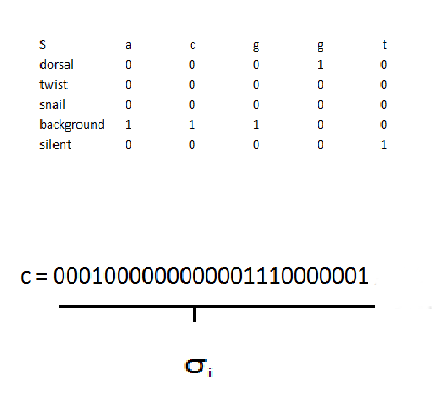
\includegraphics[width=1\textwidth]{configurationMatrixIb}\\
  \caption{The toy CRM sequence acggt is annotated at each of its loci ( positions ) to denote the configuration vector in row major ordering (1st five bits are dorsal's row, second five bits are twist's row etc...).  In the language of HMMs, the value of a configuration vector reveals the hidden state of the sequence.  Here there are 5 states, where the 'silent' state indicates a transcription factor is bound to an upstream position of the sequence, causing the loci to be covered by an internal position of the planted factor.  }\label{configurationMatrixI}
\end{figure}

Now that we have defined our configuration notation, and described the weight of a given configuration, we will explain in the next section our novel form of the pairwise interaction $\omega$ between bound factors.
%
%\begin{figure}
%  % Requires \usepackage{graphicx}
%  \includegraphics[width=1\textwidth]{1042015/HMM}\\
%  \caption{}\label{HMM}
%\end{figure}
%
%\begin{figure}
%  % Requires \usepackage{graphicx}
%  \includegraphics[width=1\textwidth]{"1042015/configuration"}\\
%  \caption{configuration or many-body state of the system}\label{configuration}
%\end{figure}

%%%%%%%%%%%%%%%%%%%%%%%%%%%%%%%%%%%%55ab

\subsection{ The pairwise interaction $\omega$ between bound factors}
%
Transcription factors often interact with each other, causing certain configurations to be more likely by decreasing the total energy of the configurations where interacting factors are jointly bound, thereby increasing the weight of those configurations.  This observation, was the physical basis behind A. Hill's famous Hemoglobin Oxygen binding model.  

In the work of Xin a number forms of distance dependent pairwise interactions between bound factors was tested, such as sinusoidal functions over space that account for 'phasing' where one bound factor interacts with the nearest neighbor that is in phase (by using the major groove distance) with the factor of interest.  Similarly, gaussian decays from the center of the planted factor, and square functions were attemted and implemented.  Hence, GEMSTAT has a small database of pariwise interaction forms.  All the forms, as ours too, only allow for interactions between nearest neighbor bound proteins. 

For the the DV network interactions between Dorsal and Twist have been experimentally shown to be distance dependent, hence we use an interaction that is a function of the DNA basepair distance separating the nearest neighbors.  For the network that we are modeling this distance dependent interaction has been shown to be dominant force driving the Dorsal border of neuroectoderm expressed genes.  For the neuroectoderm network\footnote[2]{neuroectoderm network are the set of genes coordinately expressed in the lateral regions of the developing embryo, this developing tissue spans about 10 cells at the time point under consideration}  Crocker et.al. and Szymanski et.al. \cite{pmid7774581},\cite{pmid18986212}have shown that the spacing between sites plays a dominant role in defining the number of cells that are turned on in this region (width or span of cells).

For both the DV and AP (Anterior Posterior) network short range antagonistic interactions have been show to dominate the action of repressor transcription factors\cite{pmid20087339}.  The Snail transcription factor is a short range repressor acting to regulate the DV axis, which we also model using a distance dependent interaction, commonly called 'Quenching'\cite{pmid20087339}.
\begin{figure}
  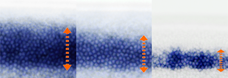
\includegraphics[width=1\textwidth]{rhoNEEs}\\
  \caption{ Changing the spacing between motifs in modules change the span of cells that are expressed.  In this Figure the spacing between two sites was adjusted by Natural Selection in orthologs of the \textit{rhomboid} gene's CRM. When the ortholog CRMs were transgenically inserted into \textit{mel} species the width of the expression pattern changes relative to the endogenous pattern width, suggesting that coopertivity between the sites is a function of the distance between sites that can be used by evolution to 'fine tune' the epression patterns in development.  When each sequence or module is expressed in its respective specie (lineage), then the relative widths (w/L where L is the lengths of the major axis of the specie's embryo, w is the width of the tissue in nanometers that express the gene) of the tissues are the same.  Different specie's embryos have different sizes hence there is a scaling law - how a characteristic (such as gene expression) changes with body size.  This Figure is from Erives Crocker et.al 2008 "Evolution acts on enhancer organization to fine-tune gradient threshold readouts. PLoS Biology"}\label{rhoNEEs}
\end{figure}

  Furthermore, since we do not know the exact form of the function, we bin the distance separating the proteins, and for each bin a free parameter is fit.  One may look for a coarse binning of the separation distance in bins of 10bp, or as fine as bins of 1bp.  If we choose the former option than an example of our protein-protein interaction parameter would be as follows:
\begin{equation}\label{}
   \overrightarrow{ \omega(d)} =  [ \omega_1 ,\omega_2 ,\ldots, \omega_b,\ldots,  \omega_n ]
\end{equation}
where the subscripts of the components of the $\omega$ vector (coopertivity or synergistic protein-protein interactions)  represent the corresponding bin ,b, ( in this case there are n bins), hence they define a bin vector, $\overrightarrow{B}$, where its components corresspond to the interval of base pair distances.

\begin{equation}\label{}
\begin{split}
 \overrightarrow{B}   &= [ B_1 ,B_2 ,\ldots, b, \ldots, B_n ] \\
     &=   [ (0-10), (11-20), \ldots,(41-50),\ldots, (x-L)]
    \end{split}
\end{equation}
Here bin b, is all interactions where two bound sites are separated by 41-50 basepairs, and x represents the last bin border, and L represents the Length of the module (sequence).  This representation of coopertivity vector, is really only useful for programming purposes, mathematically the coopertivity is simply a piecewise defined function:


\[
  \omega(d) =
  \begin{cases}
   \omega_1  & \text{ if } d \in (0,10)  \\
   \omega_2  & \text{ if } d \in (11,20)  \\
   \ \ \ \ \ \vdots \\
 \omega_n  & \text{if } d \geq x
  \end{cases}
\]

Our aim is to fit the biochemcial parameters that tune the probability of configurations that occur in live embryos.  However, we simply don't have such detailed biochemical experiments.  Hence, we use the mRNA of the target genes regulated by Dorsal Twist and Snail as a readout of what binding configurations are likely occurring, and wheter certain configurations have strong linkage (pairwise interactions) between certain bound factors.  Hence, we must infer from mRNA data, what is occuring at the DNA binding level; an expression to sequence model.  In the next section will describe a ubiquitous and obvious assumption, mRNA is caused by PolII, hence PolII binding is a proxy for gene expression.
 
\subsection{ Relating the number of mRNA transcripts to fractional occupancy of PolII }
The amount of transcription that occurs at a gene locus is encoded in two segments of DNA sequence; first, the basal promoter that binds the Basal Transcription Apparatus (BTA), which is a massive complex of many proteins including PolII; second, and most important, the CRM that binds the morphogens or distal transcription factors (such as Dorsal) that modify and remodel the chromatin state and possibly have direct linkage with the BTA.  Hence the number of mRNA transcripts can be modeled as simply a linear relationship between the number of mRNA and the fractional occupancy of a promoter sequence (which we assume includes the CRM sequence).
\begin{equation}\label{}
     \left< N_{mRNA} \right>  \propto f_{BTA}.
\end{equation}
Of course, the occupancy of the BTA, $f_{BTA}$,  is a fraction this is at most one, hence $\left< N_{mRNA} \right> $ is the average number of mRNA molecules produced per nuclear cycle normalized by the maximum production rate over a cycle. 



 

